\documentclass[../TDO4.tex]{subfiles}%

\begin{document}
\section[s]"3"{Le microscope}

\enonce{%
	Un microscope est schématisé par deux lentilles minces convergentes de même
	axe optique~: l'objectif $\Lc_1$ de centre O$_1$ et de distance focale image
	$f'_1 = \SI{5}{mm}$, et l'oculaire $\Lc_2$ de centre O$_2$ et de distance
	focale image $f'_2 = \SI{25}{mm}$. On note respectivement F'$_1$ et F$_2$ les
	foyers image de $\Lc_1$ et objet de $\Lc_2$. On appelle \textit{intervalle
		optique} et on la note $\Delta$ la distance $\obarr{F'_1F_2} = \SI{25}{cm}$.
	L'œil de l'observataire est placé au foyer image $F'_2$ de l'oculaire. On y
	visualise un objet étendu transverse AB avec A sur l'axe optique.
}%

\QR{%
Où doit se situer $A$ pour que l'œil n'ait pas à accommoder~? Répondre
en donnant l'expression et la valeur numérique de $\obarr{F_1A}$.
}{%
L'œil visant sans fatigue à l'infini, il faut que l'image par $\Lc_2$
soit à l'infini. Pour ça, l'image intermédiaire A$_1$ de A par $\Lc_1$
doit se situer dans le plan focal objet de $\Lc_2$. Autrement dit, on
doit avoir $\obarr{F'_1A_1} = \obarr{F'_1F_2}$. Ceci ce traduit
par la schématisation optique $\rm AB \opto{\Lc_1}{\rm O_1}
	\underbrace{\rm A_1B_1}_{\rm A_1 = F_2}\opto{\Lc_2}{\rm O_2} +\infty$.
On utilise donc la relation de conjugaison pour la lentille $\Lc_1$
avec origine au foyer~:
\begin{equation*}
	\obarr{FA}\obarr{F'A'} = -f'{}^2
\end{equation*}
et avec les notations choisies, $\obarr{F_1A}\obarr{F'_1A_1} =
	-f'_1{}^2$. On en tire directement
\[
	\boxed{\obarr{F_1A} = \frac{-f'_1{}^2}{\Delta}}
	\qav
	\left\{
	\begin{array}{rcl}
		f'_1   & = & \SI{5}{mm}   \\
		\Delta & = & \SI{250}{mm}
	\end{array}
	\right.
	\qso
	\xul{\obarr{F_1A} = \SI{-0.1}{mm}}\]
}%

\QR{%
	On se place dans les conditions de la question précédente. Représenter
	le trajet de 2 rayons issus de B sur une figure horizontale respectant
	le fait que $f'_1 < f'_2$. % < \Delta$ ??
}{%
	~
	\begin{center}
		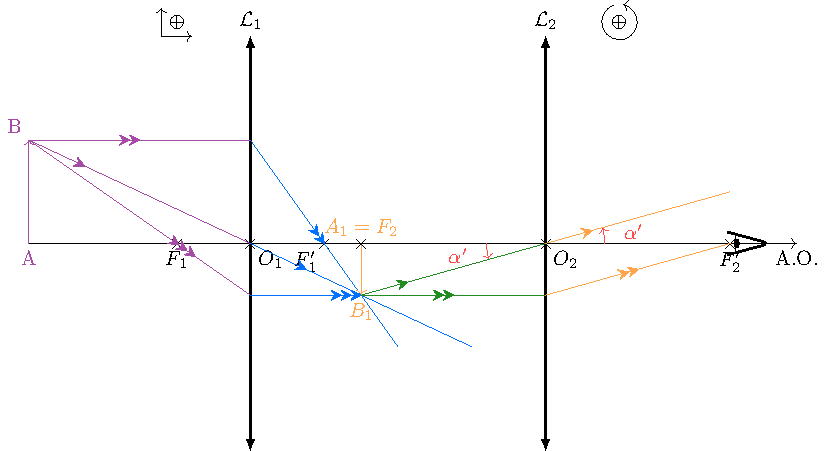
\includegraphics[width=\linewidth]{microscope.pdf}
		\label{fig:microscope}
	\end{center}
}%

\QR{%
	Soient $\alpha'$ l'angle algébrique sous lequel l'œil voit l'image
	finale de AB par le microscope, et $\alpha$ l'angle algébrique sous
	lequel il apercevrait l'objet sans microscope et à la distance
	$\Delta$. Calculer le grossissement, et interpréter son signe.
}{%
	Avec le schéma ci-dessus et dans l'hypothèse des conditions de Gauss
	($\tan\theta \approx \theta$), $\alpha' = \dfrac{\obar{\rm
				A_1B_1}}{-f'_2}$. On veut relier $\obarr{A_1B_1}$ à $\AB$ puisqu'on
	aura $\alpha = \dfrac{\AB}{-\Delta}$~: on utilise pour ça l'expression
	du grandissement avec origine aux foyers (on connaît $\obar{\rm
			F_1A}$)~:
	\begin{gather*}
		\gamma = \frac{\ABb}{\AB} = - \frac{\obarr{O_1F_1}}{\obar{\rm
				F_1A}}
		\\\Lra
		\ABb = \AB \frac{f'_1}{\obarr{F_1A}}
	\end{gather*}
	Ainsi,
	$\DS G = \frac{\alpha'}{\alpha} =
		\frac{
			-\dfrac{f'_1}{f'_2} \dfrac{\AB}{\obarr{F_1A}}
		}{
			\dfrac{\AB}{-\Delta}
		}$ donc
	\[
		\boxed{G = -\frac{\Delta^2}{f'_1f'_2}}
		\qav
		\left\{
		\begin{array}{rcl}
			\Delta & = & \SI{25}{cm} \\
			f'_1   & = & \SI{5}{mm}  \\
			f'_2   & = & \SI{25}{mm}
		\end{array}
		\right.
		\qso
		\xul{G=-500}
	\]
}%


\end{document}
